%------
% Patch
%------

\chapter*{Patchs}
\addcontentsline{toc}{chapter}{Annexe 4 : Patchs}

Le patch est le moyen d'échanger et de communiquer les modifications faites
dans le code source du noyau Linux. Ce sont des fichiers générés par commande
GIT qui font état des différences entre les lignes retirées ou ajoutées.  La
granularité des modifications de GIT est par lignes. Ainsi si une ligne a été
modifiée, GIT le verra comme si une ligne avait été retirée puis ajoutée.  \\

\noindent
+ ceci est une ligne ajoutée \\
- ceci est une ligne retirée

Un exemple de patch est montré ci-dessous.\\

\section*{Patch 4 : coresight: etm3x: Enable timestamp if supported}
\begin{figure}[H]
	\begin{center}
		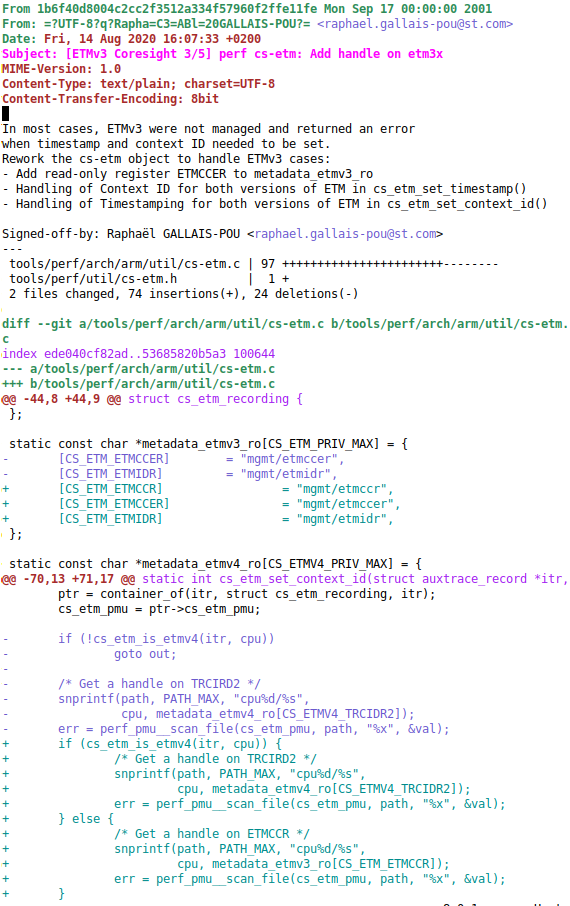
\includegraphics[width=\textwidth]{\pathPatchFour/0}
	\end{center}
\end{figure}

\begin{figure}[H]
	\begin{center}
		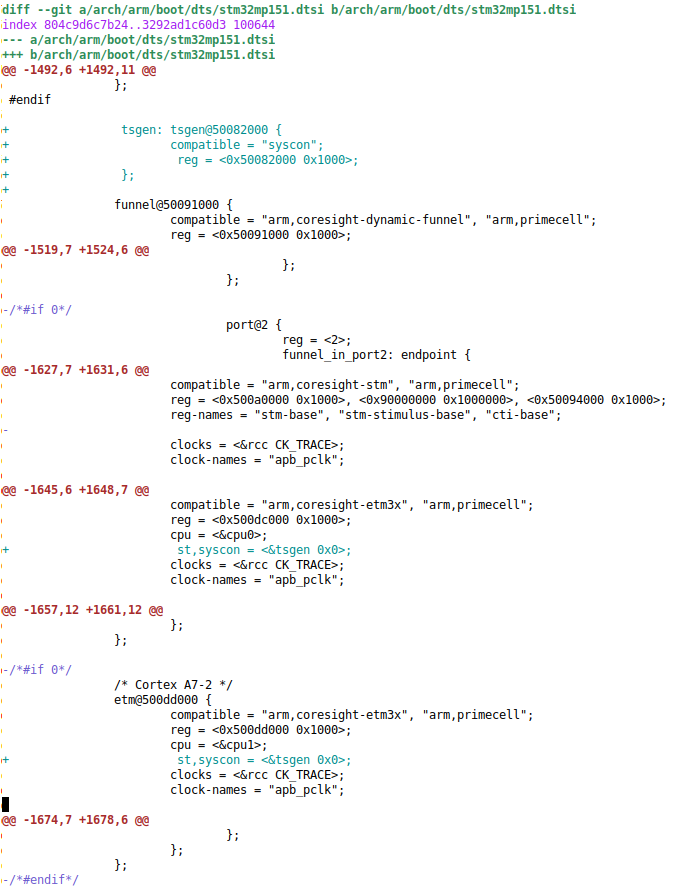
\includegraphics[width=\textwidth]{\pathPatchFour/1}
	\end{center}
\end{figure}

\begin{figure}[H]
	\begin{center}
		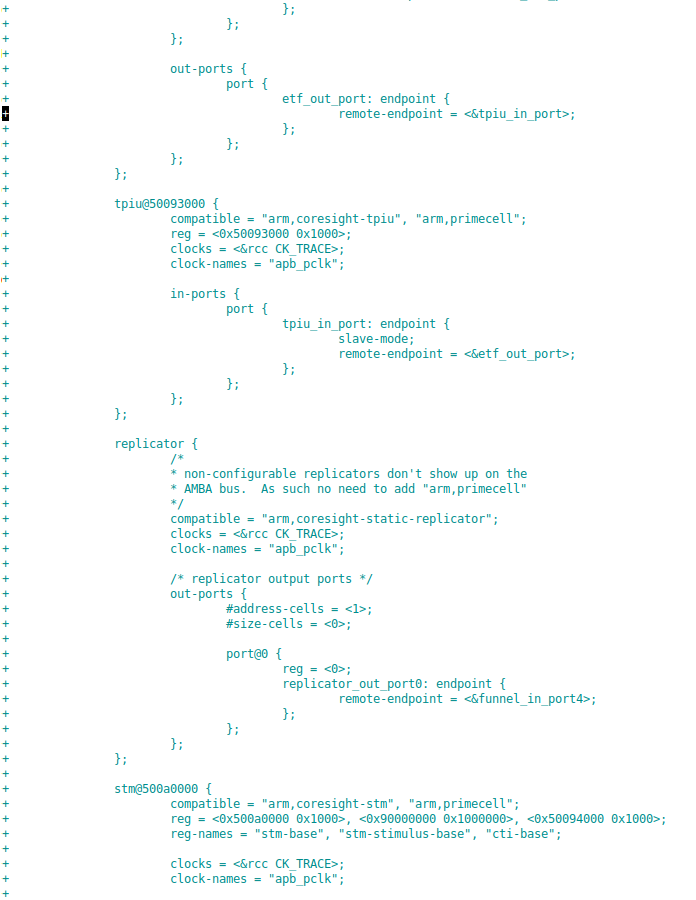
\includegraphics[width=\textwidth]{\pathPatchFour/2}
	\end{center}
\end{figure}

\begin{figure}[H]
	\begin{center}
		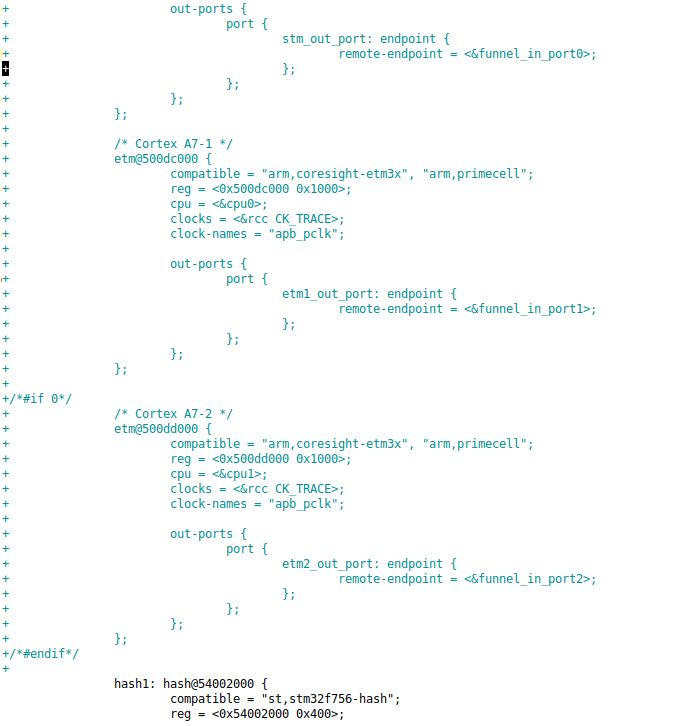
\includegraphics[width=\textwidth]{\pathPatchFour/3}
	\end{center}
\end{figure}
